\documentclass[11pt,a4paper]{article}
\usepackage[T1]{fontenc}
\usepackage{graphicx}
\usepackage{isabelle,isabellesym}
\usepackage{amssymb}
\usepackage{wasysym}
\usepackage[only,bigsqcap]{stmaryrd}
%\usepackage{masmath}

% this should be the last package used
\usepackage{pdfsetup}

\newcommand{\isasymNoMsg}{\ensuremath\varepsilon}
%\newcommand{\isasymMsg}{\texttt{Msg}}
%\newcommand{\isasymMsg}{\isatext{\rm\sffamily{}Msg}}
\newcommand{\isasymMsg}{\textsf{Msg}}
% \newcommand{\isasymB}{\textsf{B}}
% \newcommand{\isasymR}{\textsf{R}}
% \newcommand{\isasymS}{\textsf{S}}
% \newcommand{\isasymU}{\textsf{U}}
% \newcommand{\isasymW}{\textsf{W}}

\newcommand{\backslashlessgreater}[1]{\ensuremath{\backslash\!\!<}#1\ensuremath{>}}
\newcommand{\isasymHTMLNoMsg}{\backslashlessgreater{HTMLNoMsg}}
\newcommand{\isasymHTMLMsg}{\backslashlessgreater{HTMLMsg}}



\urlstyle{rm}
\isabellestyle{it}
\pagestyle{myheadings}

\begin{document}

\title{Interval Temporal Logic on Natural Numbers}
\author{David Trachtenherz}
\maketitle

\begin{abstract}
We introduce a theory of temporal logic operators using sets of
natural numbers as time domain, formalized in a shallow embedding
manner. The theory comprises special natural intervals (theory
IL\_Interval: open and closed intervals, continuous and modulo
intervals, interval traversing results), operators for shifting
intervals to left/right on the number axis as well as
expanding/contracting intervals by constant factors (theory
IL\_IntervalOperators.thy), and ultimately definitions and results for
unary and binary temporal operators on arbitrary natural sets (theory
IL\_TemporalOperators).
\end{abstract}

\tableofcontents

\begin{center}
  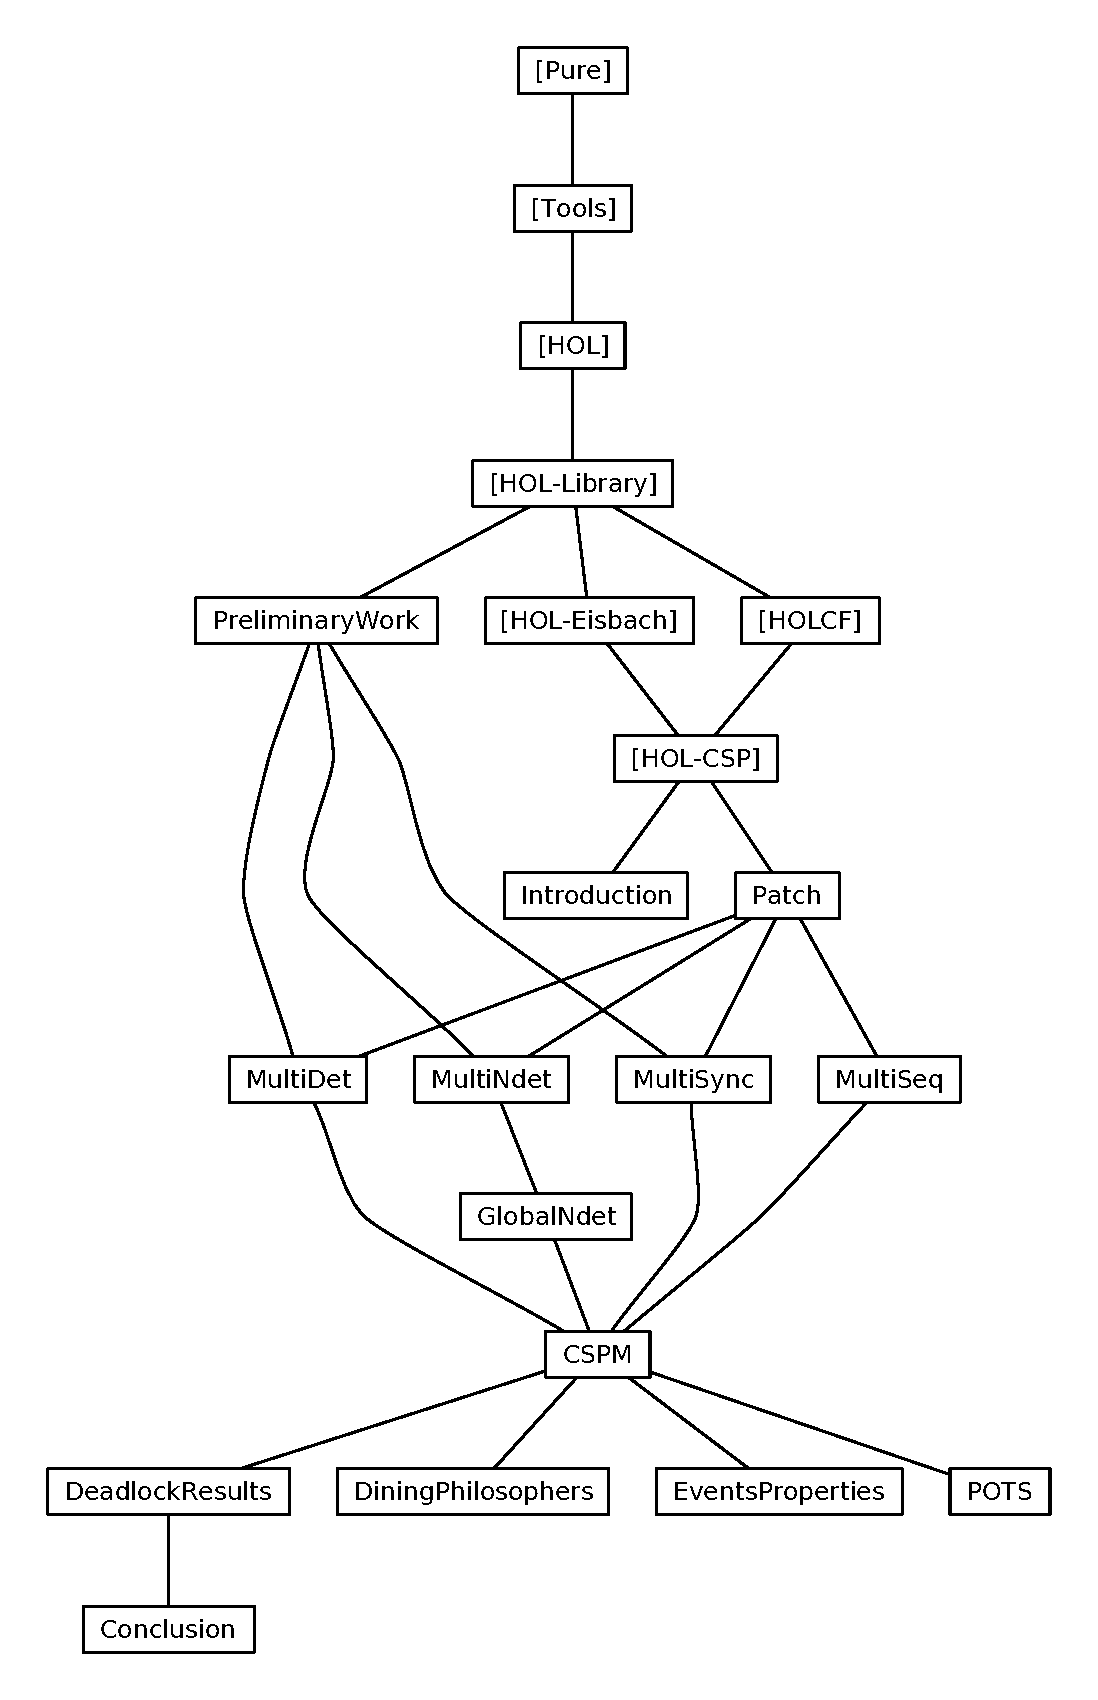
\includegraphics[scale=0.5]{session_graph}
\end{center}

\clearpage

\parindent 0pt\parskip 0.5ex
\input{session}

\end{document}
